\subsection{Parametrische Darstellung}
Den Frequenzgang erhält man, indem man die komplexe Variable $s$ durch $i\omega$ ersetzt. Das ist gleichbedeutend mit einem Schnitt der komplexen Funktion $G(s)$ entlang der imaginären Achse. Somit wird jeder Kreisfrequenz $\omega$ eine komplexe Zahl $G(i\omega)$ zugeordnet. 
\\
\\
Bedingt durch den Schnitt hat der Frequenzgang eine geringere Aussagekraft als die Übertragungsfunktion, da er nicht alle $s$ betrachtet, sondern nur die $s$, die auf der imaginären Achse liegen.
Die Bedeutung des Frequenzgangs ergibt sich aus der Tatsache, dass das stationäre Verhalten des Systems auf eine sinuidale Anregung beschrieben wird.\\
\\
Sei $u(t) = sin(\omega t)$, so ist $y_{stat}(t)$, dh. das Ausgangssignal nach Abklingen der Anfangswerte durch:
\begin{equation*}
    y_{stat}(t)=A*|G(i\omega )|sin(\omega t + \varphi (G(i\omega )))
\end{equation*}
gegeben. 

%Experimentell könnte der Frequenzgang durch die folgende Simulink-Schaltung aufgenommen werden. 
%TODO: Schaltung einfügen
%Man stellt eine Frequenz ein und schaut am Ausgang die Amplitudenverstärkung und die Phasenverschiebung an. Hat der Eingangssinus die Amplitude 1, kann ich die Verstärkung am Ausgang direkt ablesen. Den erhaltenen Punkt trägt man in das Bode-Diagramm ein. Danach wiederholt man das Experiment mit einer anderen Frequenz. Hat man genügend Punkte, so verbindet man diese und erhält das Bode-Diagramm. Ebenso wie wir an den Verläufen der Sprungantwort auf die Differentialgleichung schließen konnten, können Experten aus den Verläufen des Bode-Diagramms auf den Frequenzgang (und damit auf die Übertragungsfunktion und damit auf die Differentialgleichung) schließen.\\
%Die Phasenverschiebung kann selbstverständlich auch mit Computeralgebra ausgerechnet werden.
\subsection{Nichtparametrische Darstellung}
Experimentell kann der Frequenzgang durch folgende Simulink Schaltung simuliert werden:
\begin{figure}[H]
    \centering
    \includegraphics[width=12cm]{images_2/Frequenzgang/frequenzgang_simulink_schakltung.png}
    \caption{Frequenzgang: Simulink-Schaltung}
\end{figure}
\begin{figure}[H]
    \centering
    \includegraphics[width=10cm]{images_2/Frequenzgang/frequenzgang_simulink_plot.png}
    \caption{Frequenzgang: Plot mit Simulink}
\end{figure}
\vspace*{0.5cm}
Am Eingangssinus wird eine Frequenz eingestellt und am Ausgang die Amplituden-
Verstärkung und die Phasenverschiebung betrachtet.
Hat der Eingang die Amplitude 1, kann man die Ausgangsverstärkung direkt
ablesen.
Das Experiment wird mit verschiedenen Frequenz wiederholt und die jeweiligen
Ergebnisse werden dabei als Punkte in die folgenden beiden Diagramme eingetragen.


\subsubsection{Nyquist-Plot (Ortskurve)}
Beim Nyquist-Plot befindet sich auf der X-Achse der Realteil und auf der Y-Achse der Imaginärteil der gemessenen Punkte.
% , bei steigender Frequenz $\omega$ zu sehen
Der Plot lässt sich in Matlab mit folgendem Befehl generieren:\\
\hspace*{0.5cm}\texttt{nyquist(sys)}\\
Der dabei entstehende Plot ist in der nachfolgenden Abbildung dargestellt.
\begin{figure}[H]
    \centering
    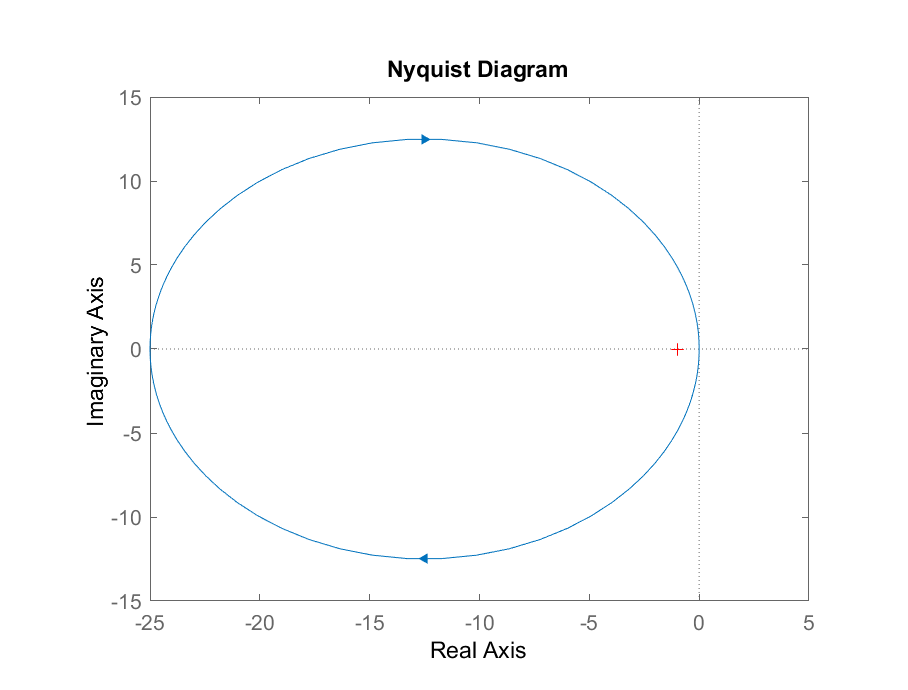
\includegraphics[width=10cm]{images_2/Frequenzgang/nyquist.eps}
    \caption{Frequenzgang: Nyquist-Plot}
\end{figure}

\subsubsection{Bode-Plot}
Das Bode-Diagramm besteht in der Praxis aus zwei einzelnen direkt untereinander dargestellten Graphen. Der obere Graph zeigt auf der y-Achse die Amplitudenverstärkung des Eingangssignals in Dezibel ($dB$). Der untere Graph zeigt auf der y-Achse die Phasenverschiebung in Grad (°) an.\\
Bei beiden Graphen befindet sich auf der x-Achse die Frequenz im Bogenmaß ($\frac{rad}{s}$).\\
In Matlab lässt sich der Bode Plot mit dem Befehl \texttt{bode(sys)} erzeugen. Das dabei erzeugte Bode-Diagramm ist auf der nachfolgenden Seite dargestellt.
\begin{figure}[H]
    \centering
    \includegraphics[width=10cm]{images_2/Frequenzgang/bode.eps}
    \caption{Frequenzgang: Bode-Plot}
\end{figure}